\documentclass[11pt,a4paper]{article}
\usepackage[a4paper,margin=22mm]{geometry}
\usepackage{graphicx}
\usepackage{subcaption}
\usepackage{float}
\usepackage{amsmath}
\usepackage{hyperref}
\hypersetup{colorlinks=true,linkcolor=black,urlcolor=blue}
\setlength{\parindent}{0pt}
\setlength{\parskip}{6pt}
\renewcommand{\baselinestretch}{1.08}

\title{\textbf{EN3160 – Assignment 02}\\Feature Detection and Image Alignment}
\author{\textbf{220701X – Savindu Wickramasinghe}\\Department of Electronic and Telecommunication Engineering\\University of Moratuwa}
\date{}

\begin{document}
\maketitle
\begin{center}
\vspace{-6mm}
{\small Repository: \href{https://github.com/Savidilsh/Fitting-and-Alignment}{\url{https://github.com/Savidilsh/Fitting-and-Alignment}}}
\end{center}

\section*{Question 1 – Blob Detection using LoG}
The Laplacian of Gaussian (LoG) filter was used to detect circular regions in the sunflower image.  
The grayscale image was smoothed with several Gaussian filters, and the Laplacian operator was applied.  
Local maxima in scale space were taken as blob centers.

\textbf{Parameters:} $\sigma_{min}=3$, $\sigma_{max}=12$, $N_\sigma=30$, threshold = 0.3.  
Only the bottom 60\% of the image was used to avoid sky detections.

The LoG correctly highlighted the main sunflower heads while ignoring small background features.  
This confirms its ability to find blob-shaped structures across multiple scales.

\begin{figure}[H]\centering
\begin{subfigure}{0.45\textwidth}
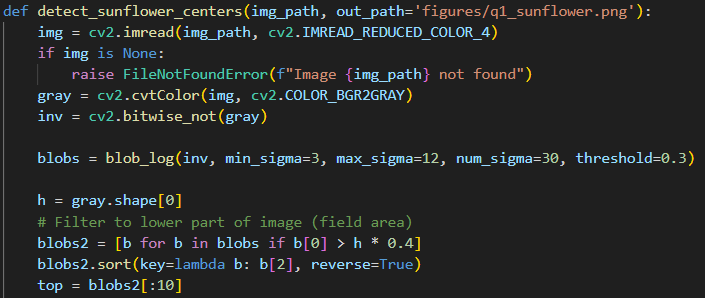
\includegraphics[width=\linewidth]{images/q1_code.png}
\caption{LoG implementation code}
\end{subfigure}\hfill
\begin{subfigure}{0.45\textwidth}
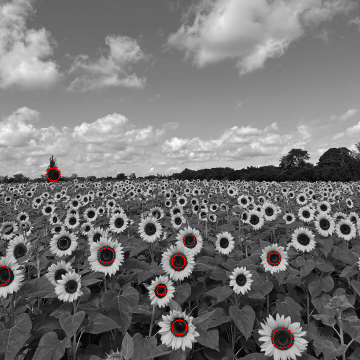
\includegraphics[width=\linewidth]{figures/q1_sunflower.png}
\caption{Detected sunflower blobs}
\end{subfigure}
\caption{Laplacian of Gaussian blob detection results}
\end{figure}

---

\section*{Question 2 – RANSAC Line and Circle Fitting}
Synthetic data combining line and circle points with Gaussian noise were generated.  
RANSAC was implemented to fit each model by sampling random points, estimating parameters, and counting inliers within a distance threshold.

\[
\text{Line: } a=-0.730,\; b=-0.684,\; d=0.992
\quad
\text{Circle: } x_0=2.083,\; y_0=2.514,\; r=10.147
\]

The estimated parameters match the true geometry closely.  
RANSAC rejected outliers effectively, giving stable estimates even in high-noise conditions.

\begin{figure}[H]\centering
\begin{subfigure}{0.31\textwidth}
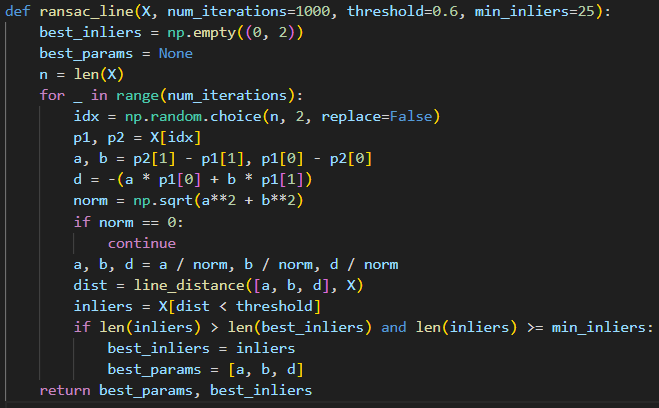
\includegraphics[width=\linewidth]{images/q2_1_code.png}
\caption{Line fitting code}
\end{subfigure}
\begin{subfigure}{0.31\textwidth}
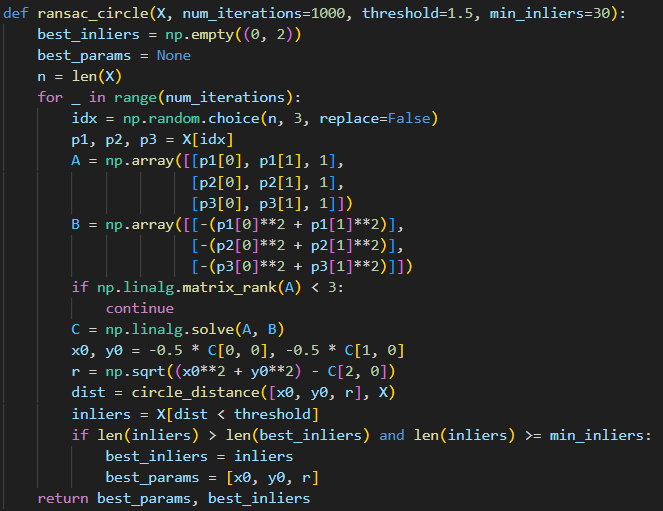
\includegraphics[width=\linewidth]{images/q2_2_code.png}
\caption{Circle fitting code}
\end{subfigure}
\begin{subfigure}{0.31\textwidth}
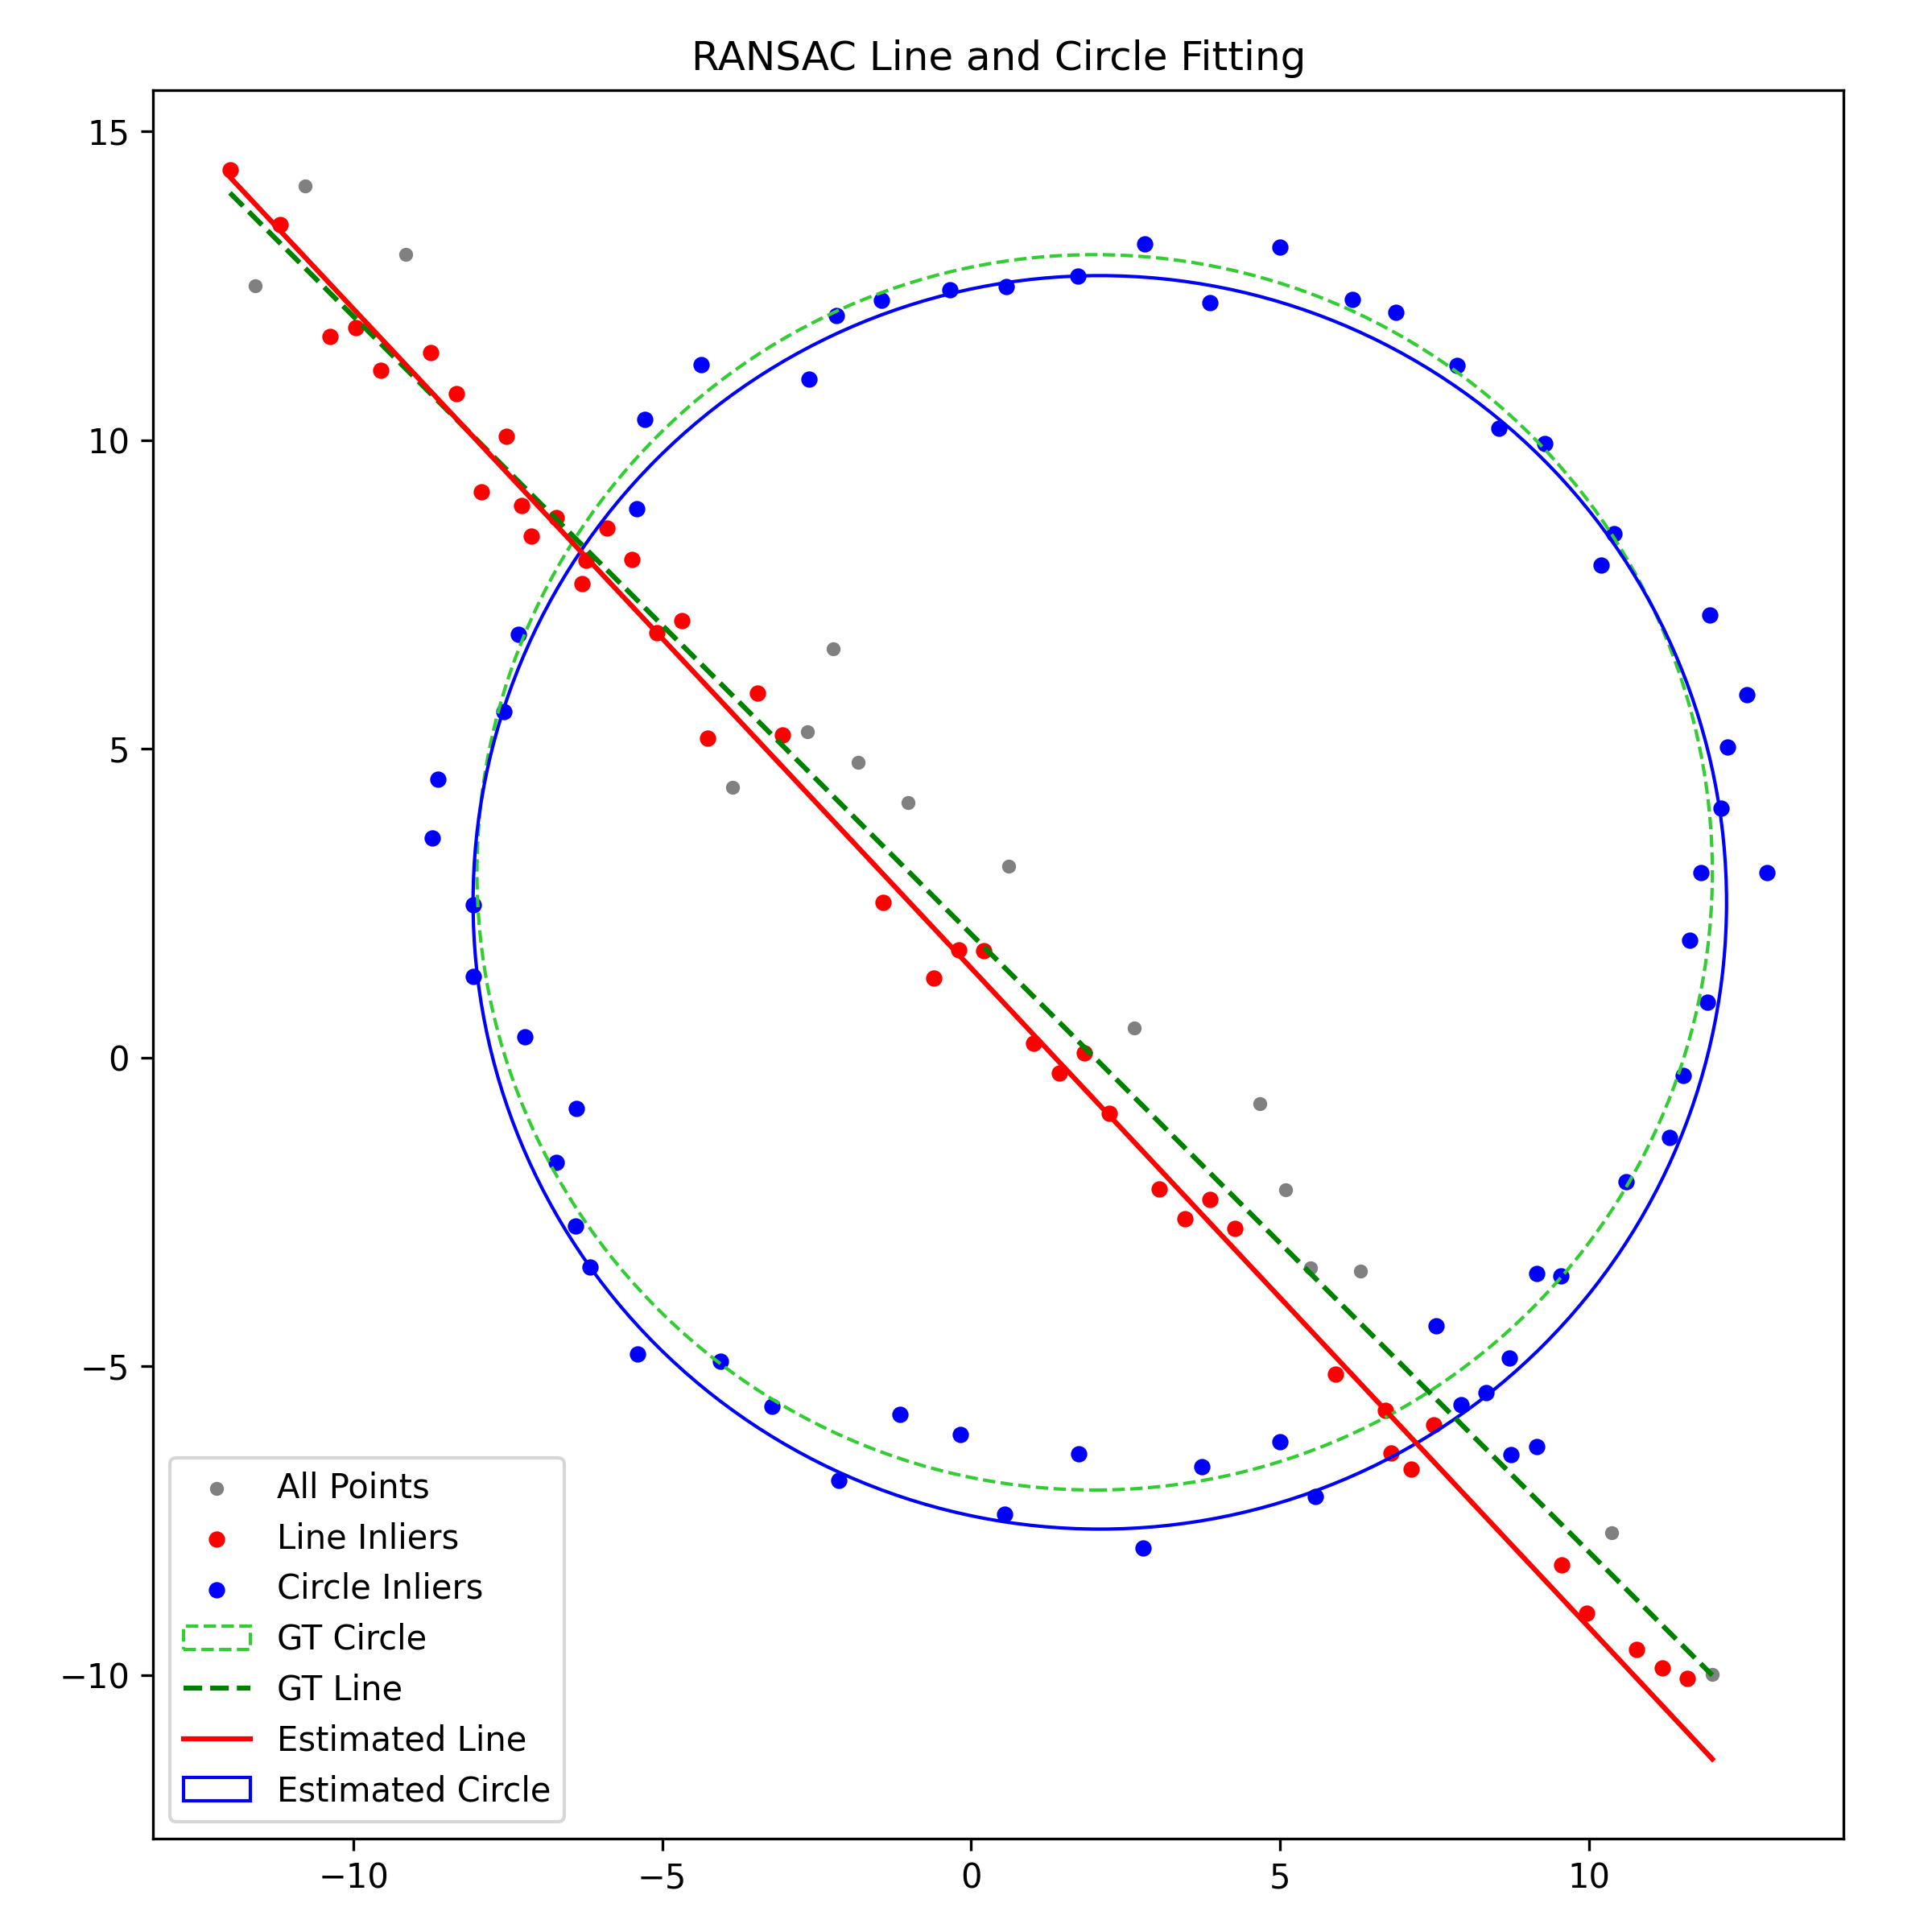
\includegraphics[width=\linewidth]{figures/q2_ransac_final.png}
\caption{Final RANSAC fit}
\end{subfigure}
\caption{RANSAC-based line and circle model fitting}
\end{figure}

When the circle is fitted first, its inliers can overlap with line points, leading to unstable results.  
Hence, estimating the line first gives better segmentation between models.

---

\section*{Question 3 – Homography Warping and Blending}
A $3\times3$ homography matrix $\mathbf{H}$ was computed from four manually selected corners on the destination image.  
It was used to warp and blend a source image onto a planar region in another image.

\textbf{Applications:}
\begin{itemize}
\item \textit{Car on billboard:} The advertisement was accurately aligned with the board edges.
\item \textit{Dog on TV:} The image was warped into the display region with correct perspective.
\end{itemize}

Both transformations appear realistic with small corner distortions due to interpolation.  
This shows how homography can create augmented-reality effects for planar objects.

\begin{figure}[H]\centering
\begin{subfigure}{0.31\textwidth}
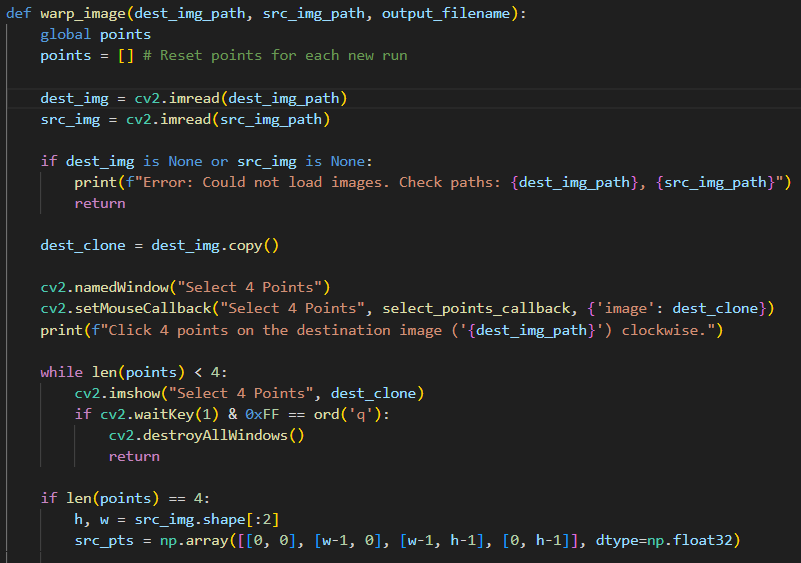
\includegraphics[width=\linewidth]{images/q3_code.png}
\caption{Homography warp code}
\end{subfigure}
\begin{subfigure}{0.31\textwidth}
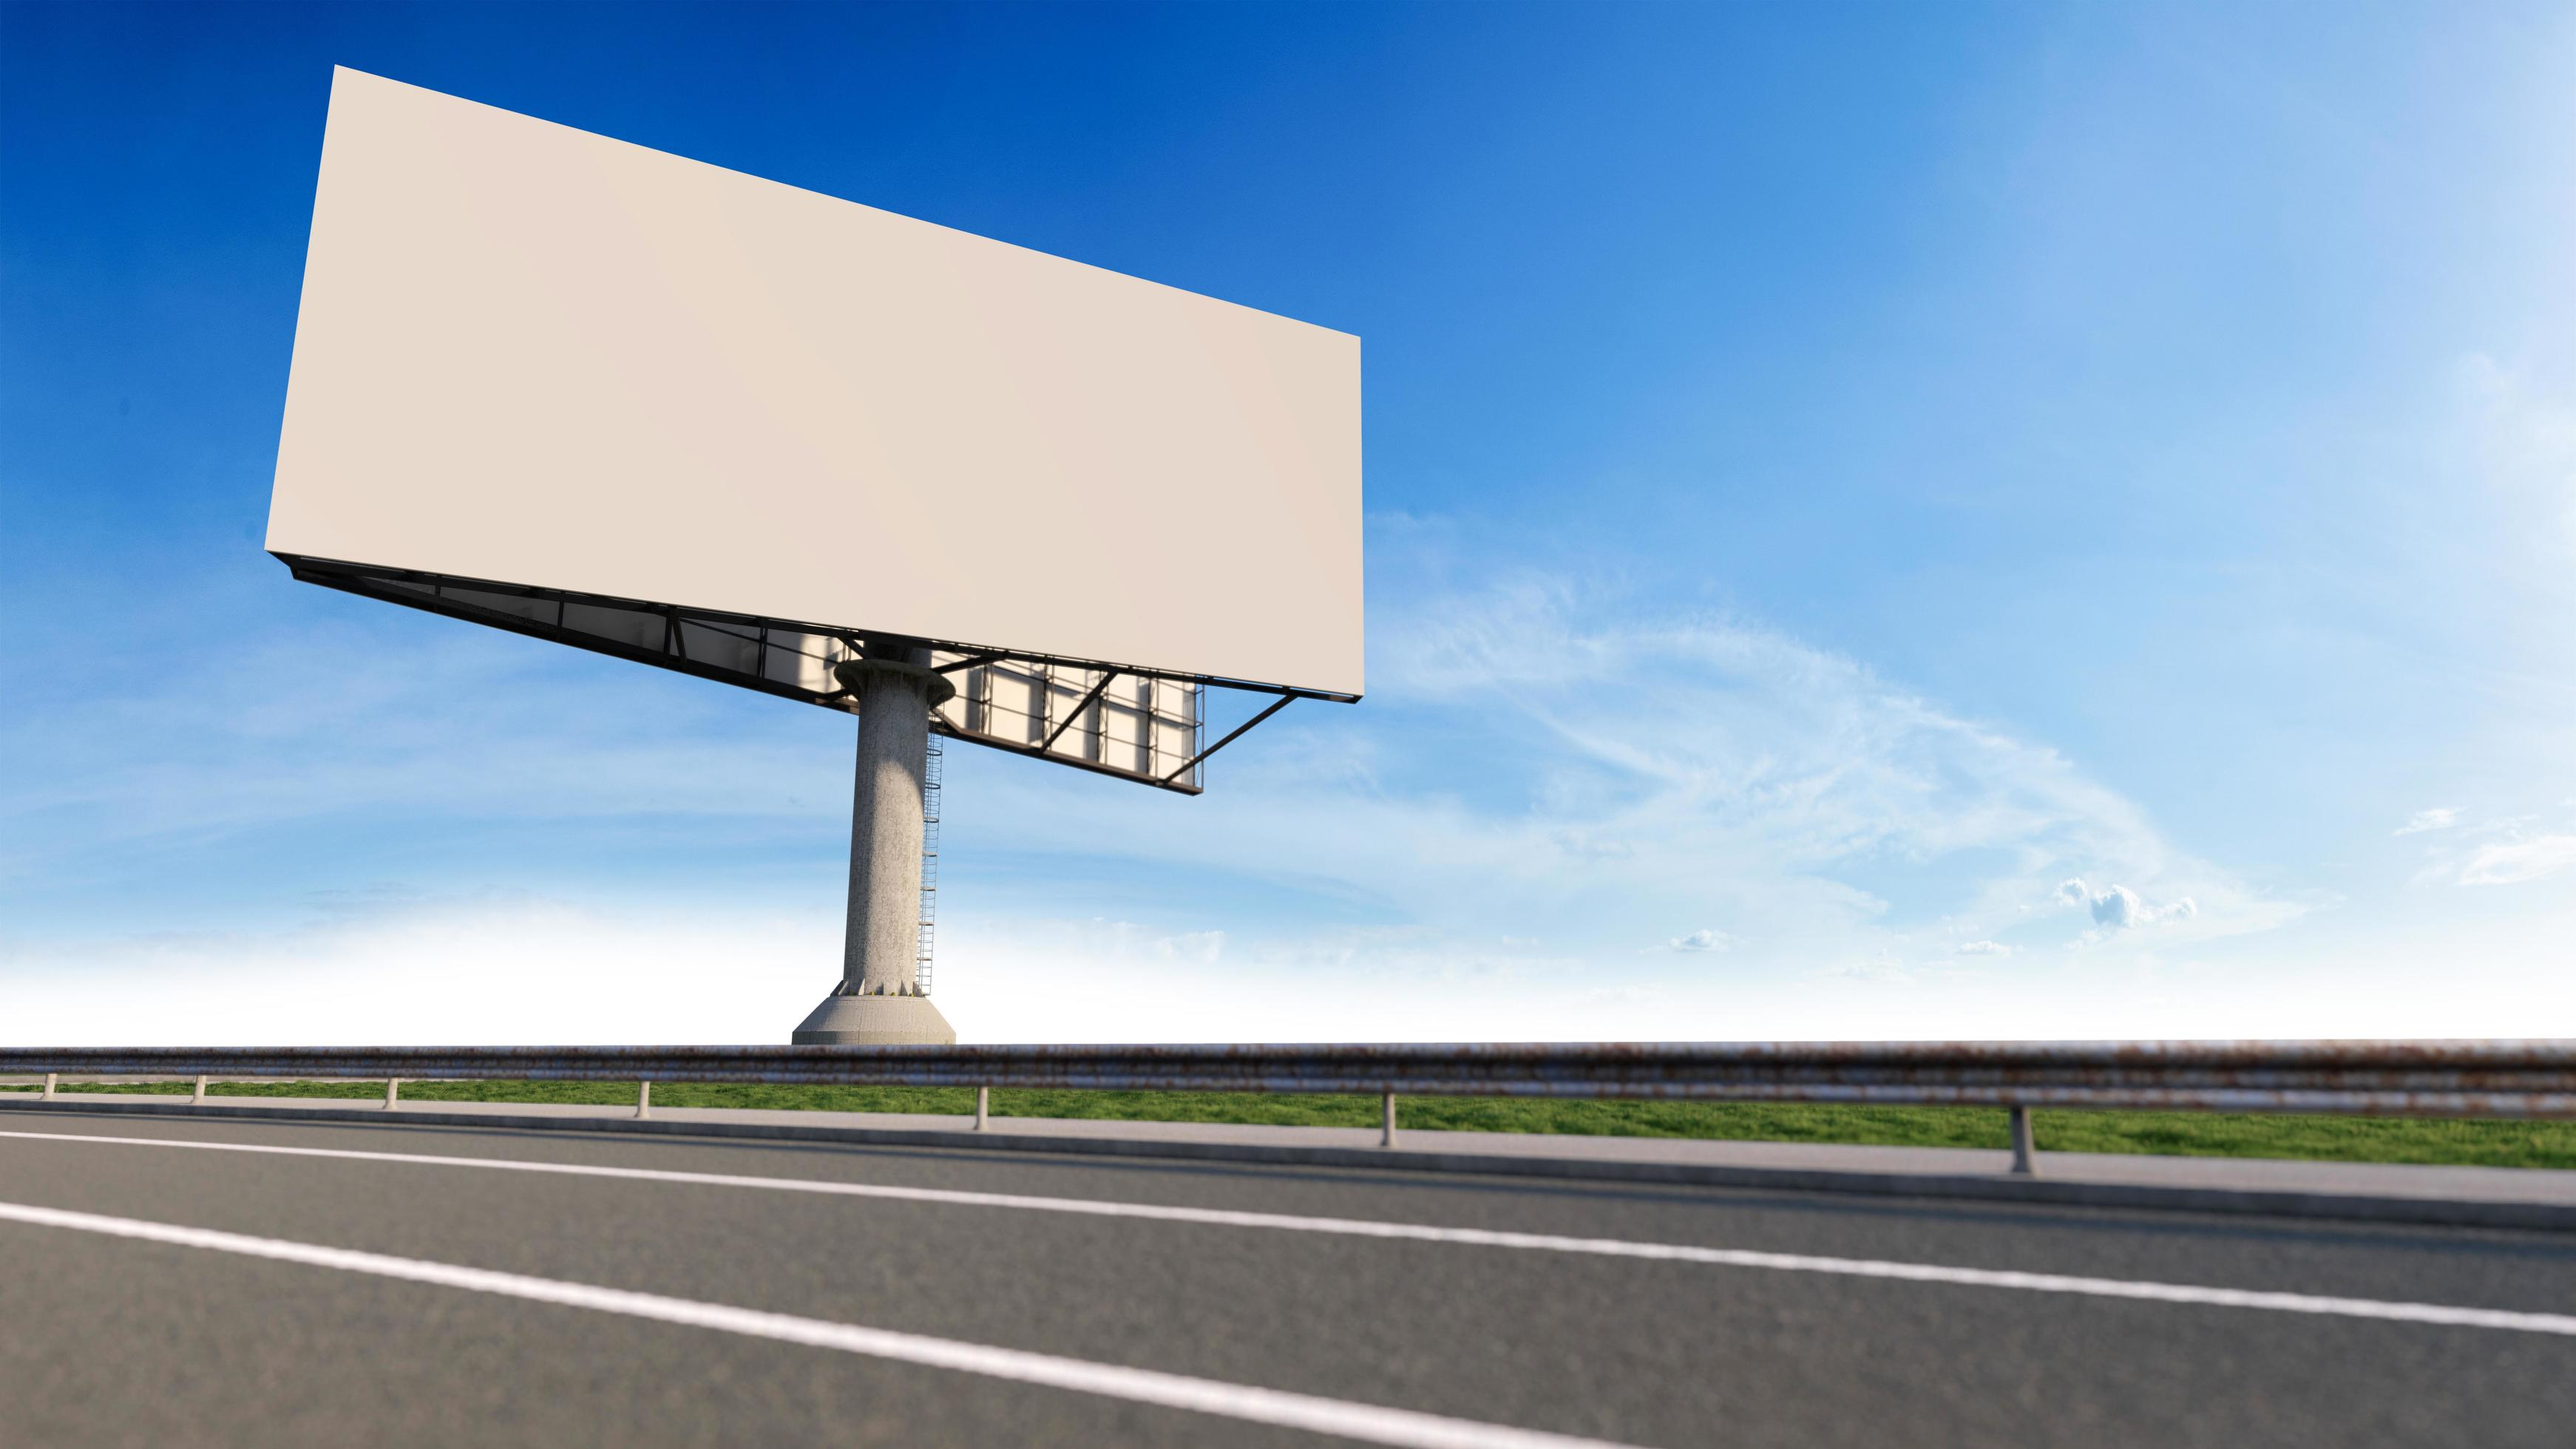
\includegraphics[width=\linewidth]{images/bill_board.png}
\caption{Car advertisement}
\end{subfigure}
\begin{subfigure}{0.31\textwidth}
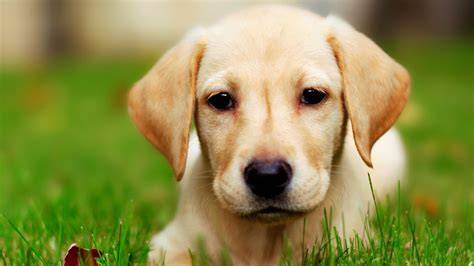
\includegraphics[width=\linewidth]{images/dog.png}
\caption{Dog on TV display}
\end{subfigure}
\caption{Perspective warping and blending results}
\end{figure}

---

\section*{Question 4 – Image Stitching using SIFT and RANSAC}
Two overlapping \texttt{graf} images (img1 and img5) were stitched using SIFT features and RANSAC.  
Keypoints were matched using Lowe’s ratio test (0.75), then filtered to remove false correspondences.  
A homography was computed from the remaining matches and used to warp and blend the images.

\textbf{Results:} 2674 (keypoints img1), 3923 (img2), 97 good matches.  
The final panorama shows smooth alignment with no ghosting.

\begin{figure}[H]\centering
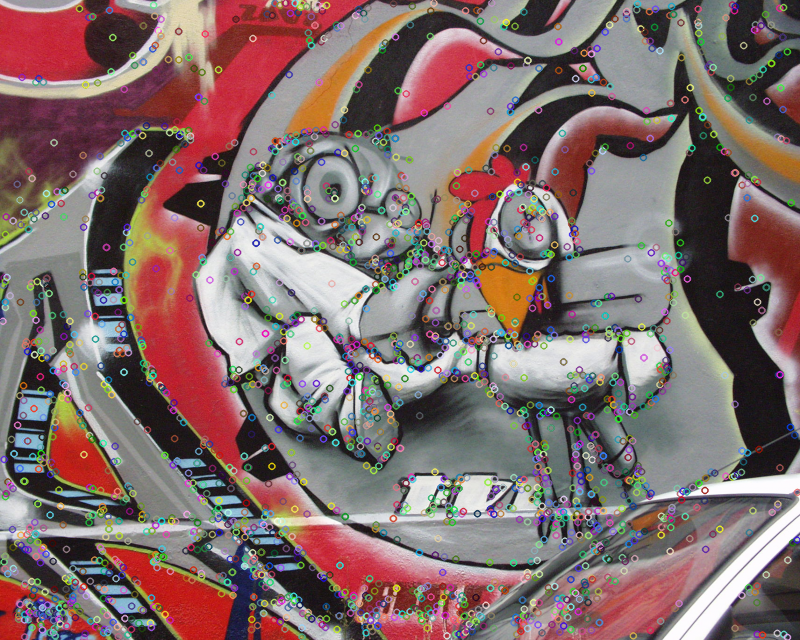
\includegraphics[width=0.31\linewidth]{figures/q4_keypoints_img1.png}
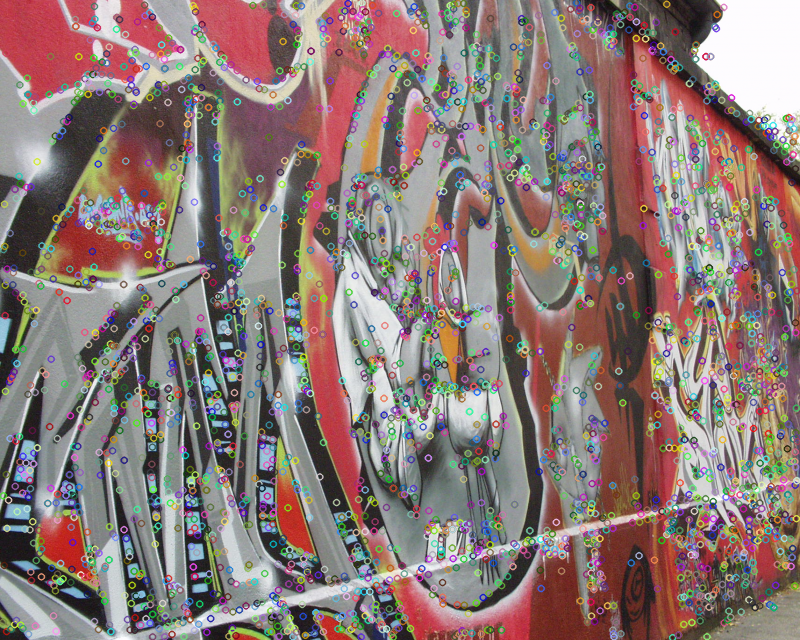
\includegraphics[width=0.31\linewidth]{figures/q4_keypoints_img2.png}
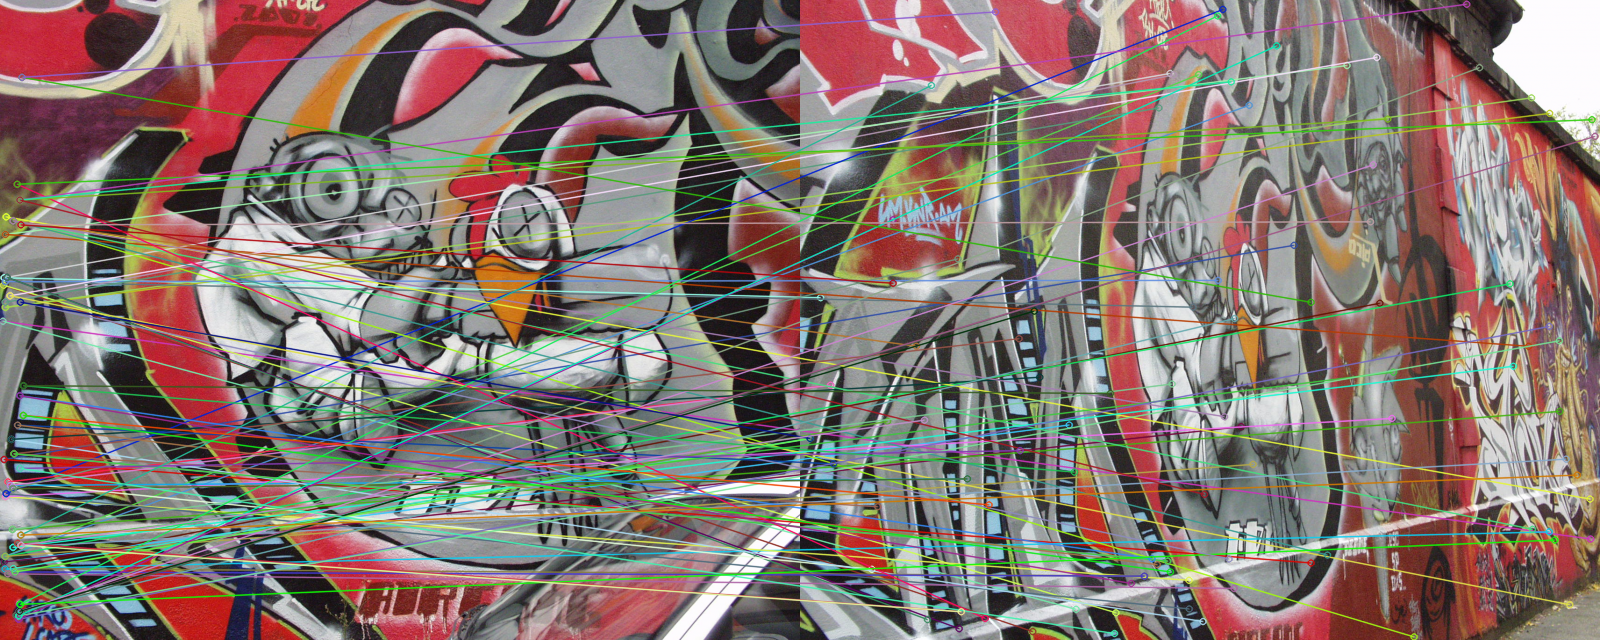
\includegraphics[width=0.31\linewidth]{figures/q4_initial_matches.png}

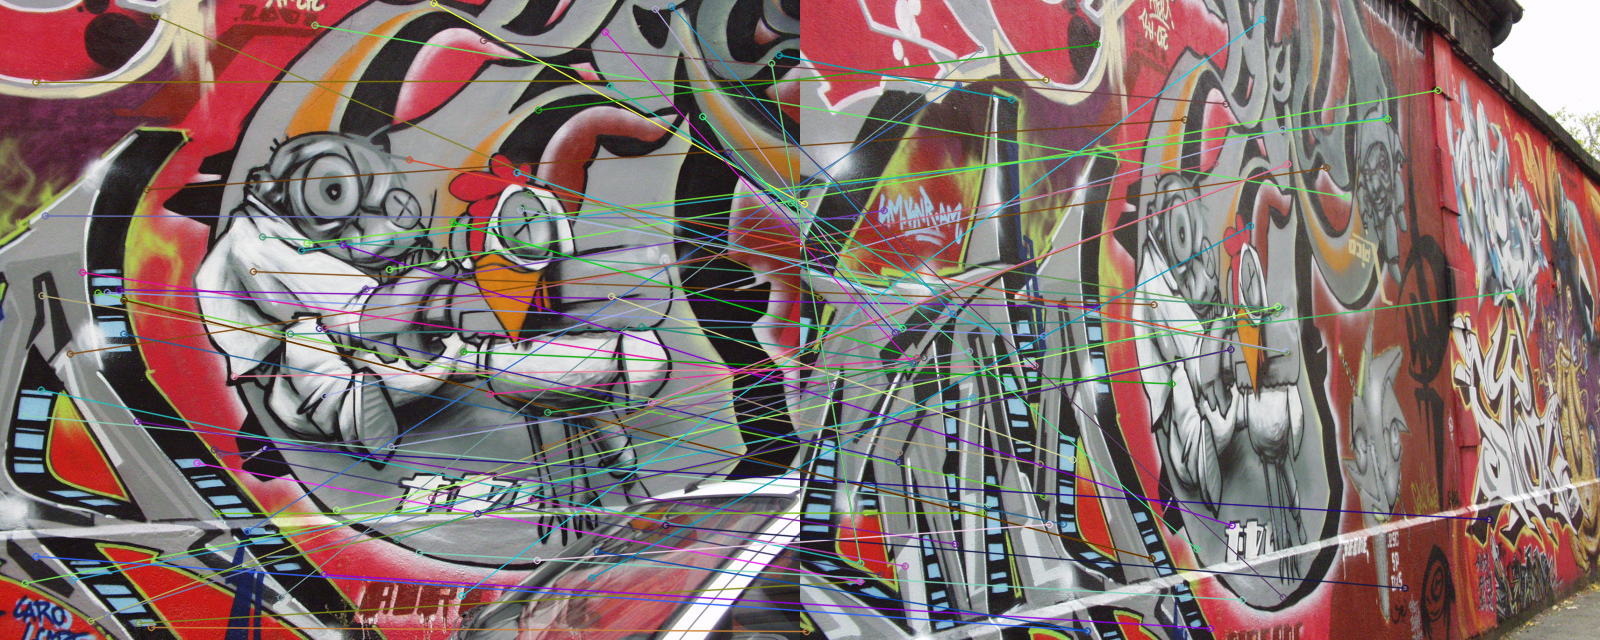
\includegraphics[width=0.46\linewidth]{figures/q4_good_matches.png}
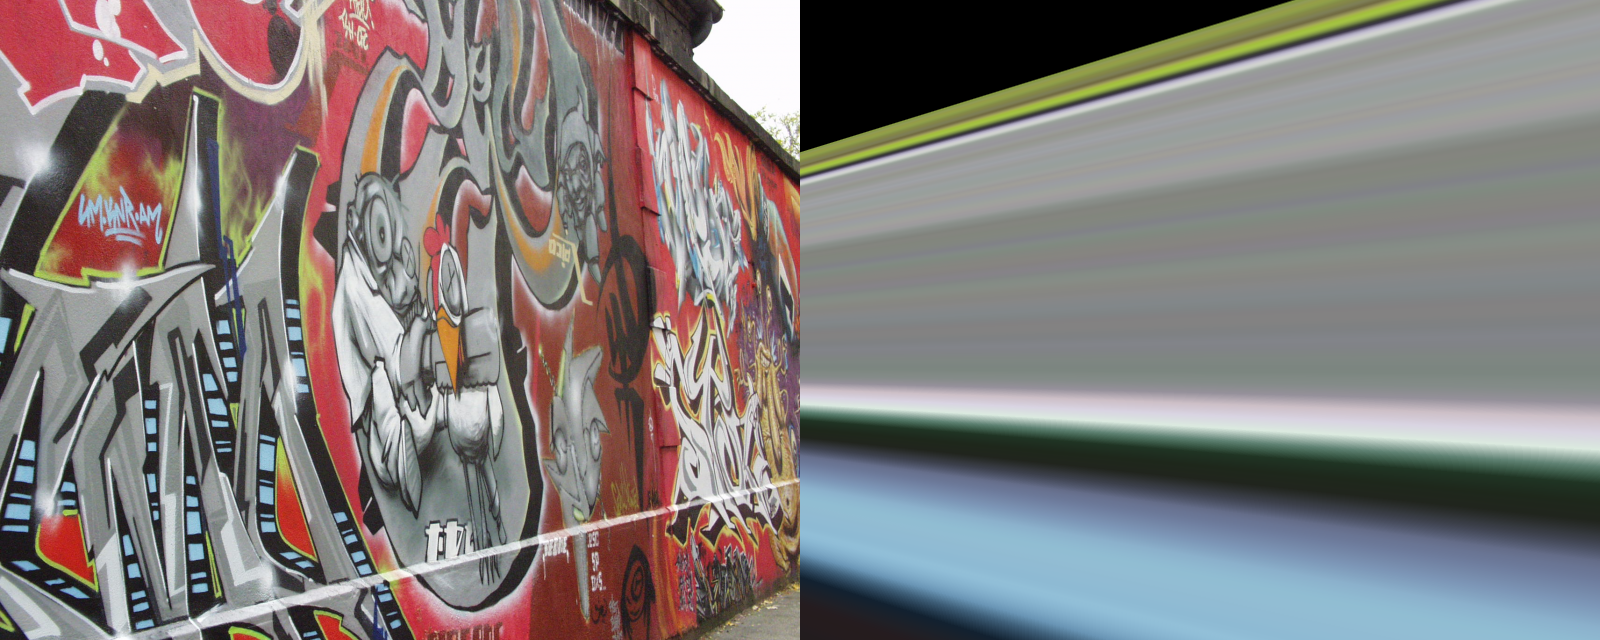
\includegraphics[width=0.46\linewidth]{figures/q4_stitched_panorama.png}
\caption{SIFT keypoints, filtered matches, and final stitched panorama}
\end{figure}

The combination of SIFT and RANSAC proved robust for feature-based alignment. SIFT ensured repeatable keypoints under scale and rotation, while RANSAC eliminated false matches to produce accurate homography estimation.

---

\section*{Conclusion}
This assignment demonstrated the core ideas of feature detection, robust model fitting, and geometric alignment.

\begin{itemize}
\item \textbf{LoG:} Detected circular sunflower heads at multiple scales.  
\item \textbf{RANSAC:} Recovered accurate line and circle models despite noise.  
\item \textbf{Homography:} Enabled realistic planar warps for scene integration.  
\item \textbf{SIFT + RANSAC:} Produced a clean and accurate stitched panorama.
\end{itemize}

All four sections together fulfil the requirements of EN3160 Assignment 02 on Fitting and Alignment.  
The methods implemented show how feature-based vision techniques can be used for object detection and scene reconstruction in practical applications.

\end{document}
